\title{\LARGE{Exercise Sheet 0x02}\\%
\Large{PSI-AdvaSP-M: Advanced Security and Privacy}
}
\author{
Barbara Hoffmann (1759786)\\
Sascha Riechel (1740803)\\
Isabell Sailer (1863490)\\
Tobias Schwartz (1738195)\\
}

\date{Submitted: \today\\%
Token for late submission is being used}

\documentclass[12pt]{article}
\usepackage{graphicx}

\begin{document}
\maketitle


\section{Task 1}\label{task1}
In the pcap file we found a packet that uses the Simple Service Discovery Protol, where the USER-AGENT is specified as Google Chrome, as depicted in Figure~\ref{wireshark_evidence}.
\begin{figure}[h]%
\centering%
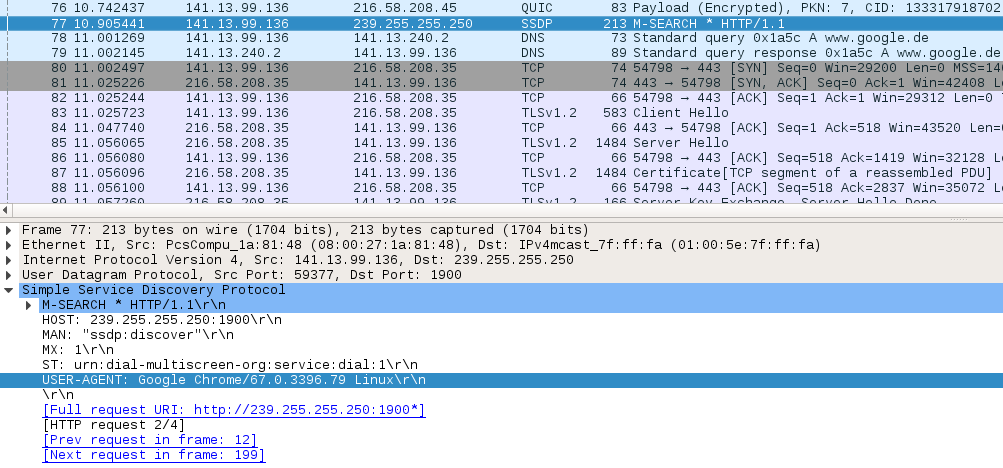
\includegraphics[width=\textwidth]{images/task_1_evidence_browser.png}%
\caption{Wireshark local traffic observation of browser}%
\label{wireshark_evidence}%
\end{figure}%



\section{Task 2}\label{task2}
To view only the traffic inside the local network, we employ a display filter in wireshark to show only traffic within the subnet of our own IP-address. We choose 141.13.99.0/24 as this filter. An excerpt of the filtered traffic can be seen in Figure~\ref{img_wireshark_overview}.

\begin{figure}[h]%
\centering%
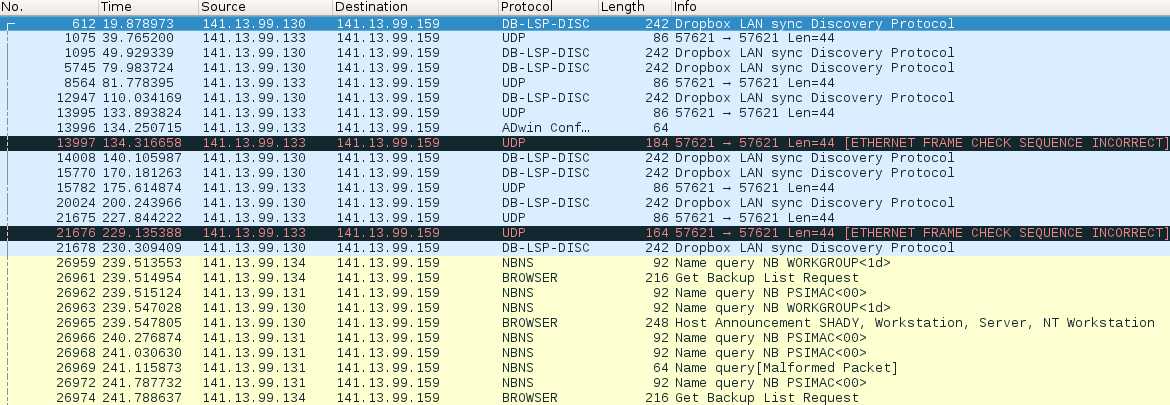
\includegraphics[width=\textwidth]{images/wireshark_overview.png}%
\caption{Wireshark local traffic observation}%
\label{img_wireshark_overview}%
\end{figure}%

We can see a dropbox service running and mainly NBNS and BROWSER traffic broadcasted in the local network. As an example we analyze one of the BROWSER pakets (see Figure~\ref{img_wireshark_browser}).
A host with name "SHADY" running Windows 7 or Windows Server 2008 R2 is available on IP-address 141.13.99.130.

\begin{figure}[h]%
\centering%
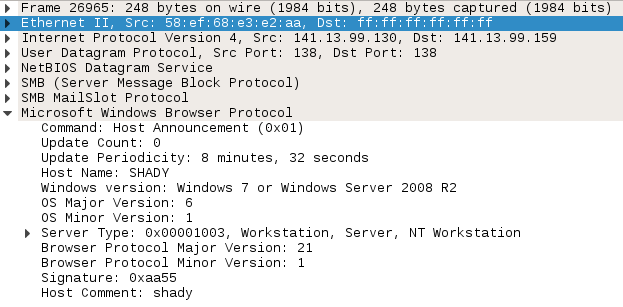
\includegraphics[width=\textwidth]{images/wireshark_browser.png}%
\caption{Wireshark BROWSER packet analysis}%
\label{img_wireshark_browser}%
\end{figure}%

Additionally, we are able to retrieve a GeoIP entry stating that all examined packets were issued in Bamberg by the ``Verein zur Foerderung eines Deutschen Forschungsnetzes e.V." (see Figure~\ref{img_wireshark_geoip}).

\begin{figure}[h]%
\centering%
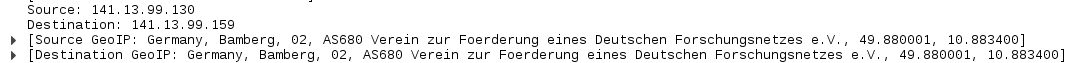
\includegraphics[width=\textwidth]{images/wireshark_geoip.png}%
\caption{Wireshark GeoIp observation}%
\label{img_wireshark_geoip}%
\end{figure}%

\newpage
\section{Task 3}\label{task3}
We implemented a python script to translate the given list of 80 websites into their corresponding .pcap files using tcpdump. Using a different script we are able to retrieve the histograms and store them in a matrix for later comparison.
Unfortunately, we ran out of time while implementing the splitting of the given .pcap traffic flow into appropriate chunks and comparing them to the earlier computed histograms.

Therefore we were not able to complete this and all further tasks. We would like to continue working on the assignment, if a late submission is still credited. Thus, we use our late submission token for this assignment.  
\end{document}
